\scanpage{118}

\diagram{$i\leq n-1\qquad
\begin{array}{l|cccc|}\text{poids}&0&1&\hspace{3em}&2i\\\hline
\text{niveaux}&0&1&&2i\\\hline\end{array}$}

\diagram{$E_2^{i\,0}\qquad
\begin{array}{l|c|c|c|c|}\text{poids}&\unsure{0}&1&&i\\\hline
\text{niveau }\leq&0&1&&i\\\hline\end{array}$}

\diagram{$E_2^{i-1\,1}\qquad
\begin{array}{l|c|cc|c|c|}\text{poids}&2&3&&i&i+1\\\hline
\text{niveau}&0&1&&i-2&i\deleted{\unsure{+2}}\unsure{-1}\\\end{array}$}

\margin{\deleted{\unsure{car}}\quad \deleted{$p+q=i$}}

\diagram{$E_2^{\unsure{(i-2),2|i-2,2}}\qquad
\begin{array}{l|c|c|c|c|c|c|}\text{poids}&4&5&\diagup\!\diagup&i&i+1&\deleted{\unsure{2}}i+2\\\hline
\text{niveau}&0&1&\diagup&i-4&i-3&i-2\end{array}$}

\margin{\deleted{$p\leq \unsure{2}(n-1-q)$}\quad \deleted{$p+q\leq n-1$}\quad $i\deleted{\unsure{+q\leq}}$}

\diagram{$E_{\deleted{\unsure{*}}2}^{0\,i}\qquad
\begin{array}{l|c|}\text{poids}&2i\\\hline \text{niveau}&0\end{array}$}

\diagram{\tikz[baseline=(a.base)]\node[draw,ellipse,inner sep=2pt](a){$i\leq n-1$};\quad
$\boxed{\begin{array}{l|c|c|c|c|c|c|c|c|}\text{poids}&0&1&\cdots&i-1&i&i+1&\cdots&2i\\\hline
\text{niveau}&0&1&&i-1&i&i-1&&0\end{array}}$}

\diagram{\tikz[baseline=(a.base)]\node[draw,ellipse,inner sep=2pt](a){$i\geq n$};\quad
\uuline{$E_2^{i\,0}$}\quad $
\begin{array}{|c|c|c|c|c|c|}2(i-n+1)&2(i-n+1)+1&\cdots&-&\deleted{\unsure{i-1}}&i\\\hline
0&1&2&&\deleted{\unsure{i}}&2(n-1)-i\end{array}$}

\diagram{$E_2^{i-1,1}\qquad
\begin{array}{|c|c|cc|c|c|}2(i-n)+2&2(i-n)+3&&\hspace{1em}&i&i+1\\\hline
0&1&&&2n-i-2&2n-i-\unsure{1|2}\end{array}$}

\diagram{$E_2^{i-2,2}\qquad
\begin{array}{|c|c|c|c|c|c}2(i-n)\deleted{\unsure{+3}}+4&2(i-n)+\unsure{3|5}&&i&i+1&i+2\\\hline
0&1&&2n-i-2&2n-i-3&2n-i-2\end{array}$}

\diagram{$E_2^{i-3,3}\qquad
\begin{array}{|c|c|c|c|c|c|c}2(i-n)+6&2(i-n)+7&&i&i+1&i+\unsure{3|2}&i+3\\\hline
0&1&&2n-i-6&2n-i-5&2n-i-4&2n-i-3\end{array}$}

\deleted{$E$}

\diagram{$E_2^{0\unsure{;|,}i}\qquad \begin{array}{|c|}2i\\\hline 0\end{array}$}

\figure{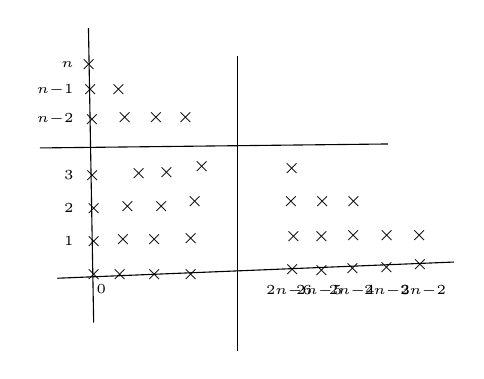
\begin{tikzpicture}[x=.44cm,y=.42cm]
\draw (0,-1.45)--(-.15,7.45); \draw (-1.05,-.11)--(10.4,.38);
\draw (-1.55,3.83)--(8.5,3.95); \draw (4.15,-2.3)--(4.15,6.6);
\foreach \x/\y in {0/0,.75/0,1.75/0,2.8/0,5.73/.14,6.58/.13,7.47/.17,8.45/.21,9.42/.30,0/1,.85/1.07,1.75/1.07,2.80/1.10,5.77/1.15,6.58/1.16,7.49/1.18,8.46/1.18,9.4/1.19,0/2,.98/2.04,1.95/2.05,2.92/2.20,5.7/2.20,6.6/2.20,7.5/2.22,-.04/3,1.30/3.05,2.10/3.07,3.12/3.25,5.72/3.20,-.05/4.69,.90/4.75,1.80/4.74,2.65/4.75,-.1/5.58,.72/5.60,-.14/6.35}{\node[inner sep=0pt] at (\x,\y){$\scriptstyle\times$};}
\foreach \y/\lab in {1/1,2/2,3/3,4.69/{n-2},5.58/{n-1},6.35/n}{\node[left] at (-.3,\y){$\scriptscriptstyle\lab$};}
\foreach \x/\lab in {.22/0,5.64/{2n-6},6.51/{2n-5},7.45/{2n-4},8.47/{2n-3},9.51/{2n-2}}{\node[below] at (\x,-.02){$\scriptscriptstyle\lab$};}
\end{tikzpicture}}

\[ \unsure{1} \]

\[
\begin{aligned}
q&=2n-i\qquad p=2(i-n)\\
E_2^{2(i-n),2n-i}&=\mathbb R^{2(i-n)}f_{Z}(\mathbb Q_\ell\\
&\phantom{={}}2(i-n)+2(2n-i)=2n
\end{aligned}
\]

% archive sheet number: 117
